\documentclass[t]{beamer}


\usepackage[T1]{fontenc}
\usepackage[utf8]{inputenc}
\usepackage[ngerman]{babel}
\usepackage[babel,german=quotes]{csquotes}
\usepackage{graphicx}

\usepackage{wasysym} % Fuer den Blitz :-)

\usetheme{fau-i12-4-3}
%\usetheme[clean]{fau-i12-4-3} % you can also use option clean to get rid of header and footer

% Title page
%\title{Kurztitel}{Voller Titel}

\title[$\sqrt 2 \not\in \mathbb Q$]{$\sqrt 2$ ist irrational}
\subtitle{--- Zur Unvollständigkeit von $\mathbb Q$ ---}

\author[Wanka et al.]{Rolf Wanka\inst{1} \and Pythagoras\inst{2}
\and Michael Gla\ss}

\date[STACS 12]{Symposium on Theoretical Aspects of Computer Science,
February 2012, Irgendwo in Frankreich}

\institute[FAU \&{} Kroton]{\inst{1}University of Erlangen-Nuremberg,
Computer Science Department
\and
\inst{2}Schule zu Kroton in Unteritalien}

\begin{document}

\frame[plain,c]{\titlepage} % plain-Option deaktiviert Kopf- und Fusszeile

\section{Jetzt kommt ein Beweis}

%--------------------------------------------------
\begin{frame}
\frametitle{Ein Widerspruchsbeweis}

\pause

\begin{enumerate}
\item Annahme:
      {\color{red}$\sqrt 2 \in \mathbb Q$}\pause, also
      {\color{red}$\sqrt2=\dfrac a b$} \pause
      für $a,b\in \mathbb N$ und $a$ und $b$
      teilerfremd. \pause
\item Also umgeformt: {\color{red}$2=\dfrac{a^2}{b^2}$}\pause,
      und damit {\color{red}$2\cdot b^2=a^2$}.\pause
\item Damit muß $a^2$ gerade sein\pause, und also gilt:
      {\color{blue}$a$ ist durch $2$ teilbar}.\pause

      D.\,h.: {\color{red}$a=2\cdot k$} für  ein $k\in\mathbb N$.\pause
\item Somit haben wir mit Zeile 2:\quad
      {\color{red}$2\cdot b^2=4\cdot k^2$} \pause
      bzw.  {\color{red}$b^2=2\cdot k^2$}\pause
\item Wie in Zeile 3 folgt jetzt auch:
      {\color{blue}$b$ ist durch $2$ teilbar}.\pause
\item {\color{blue}$a$ und $b$ sind also beide durch $2$} teilbar\pause, also
      \textbf{nicht} teilerfremd.\pause
\item {\color{red}\begin{Huge}\lightning\end{Huge}} \pause
      Widerspruch zu Zeile 1.\pause
\end{enumerate}

 Also gilt: {\color{red}$\sqrt 2 \not\in \mathbb Q$}

\end{frame}
%--------------------------------------------------

\section{Jetzt kommen noch zwei Bilder}

%--------------------------------------------------

\begin{frame}
\frametitle{Mit Kopf- und Fußleiste}

Den Beweis fanden seine wissenschaftlichen Nachkommen
im 5.~vorchristlichen Jahrhundert:\pause

\bigskip

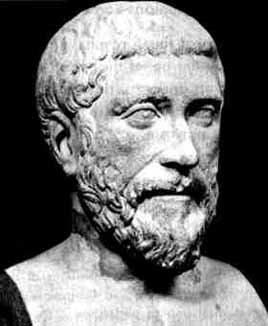
\includegraphics[height=7cm]{pythagoras.jpg}

Pythagoras (570 v. Chr. bis nach 510 v. Chr)\pause

\textbf{Und jetzt noch eine Folie ohne Kopf- und Fußleiste}

\end{frame}
%--------------------------------------------------

\frame[plain,c]{

\begin{center}
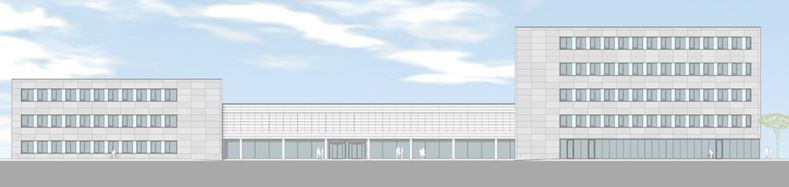
\includegraphics[width=20cm]{neubau.png}

\pause

\bigskip

Und nun zur Schlußfolie
\end{center}
}
%--------------------------------------------------

\section{Vielen Dank fürs Durchblättern!}

\end{document}
